% Chapter 1

\part{Exploring market behavior with inverse simulation} % Main chapter title
This part will cover the methods used in trying to link the various model parameters to different kinds of market behavior. The model has several parameters which must be selected carefully before the simulation can be used to infer knowledge about market behavior. The main focus is on the influence of the fast trader latency parameters.

The model must be calibrated such that it mimics the behavior of real markets. Since virtually every aspect of the simulation behavior depends on the values on the parameters, these must be chosen carefully in order for the simulation to produce ``realistic'' behavior, i.e.,	behavior that have could be found to occur in real markets. The way in which this was accomplishes in this work can be divided into four rough stages, which are outlined in the next section. 

The process of selecting parameters turned out to consume a significant amount of time, and simply using a genetic algorithm to optimize over the entire space of parameters was not enough. Instead, the process was a slow and iterative one of running the genetic algorithm to create a data set, analyze the data set to find out what was discovered in the search, and then run the genetic algorithm again with different parameters. Thus several data sets were created, each with the purpose of examining some aspect of the simulation, or of the parameter tuning method itself. 

%The fact that the model is capable of reproducing market with dynamics which is unlikely to be observed in real-world markets does not mean that the model is inherently bad. 

%A model which will only occasionally reproduce realistic market behavior might be considered as bad, 

%Just as 


%Rather, since the model has a large number of parameters, the appropriate range of which cannot be determined a priori, 






%

%The parameter tuning has two overall goals, which are covered in the following section.





\section{Overall procedure}\label{section:motivation_and_procedure}
The selection of parameters is a fairly complicated process because of the large parameter space, and because it takes a significant time to evaluate the fitness of a given set of parameters\footnote{The calculation time depends largely on the parameters, such as the number of agents and how active these are. Typically one to several minutes are required to evaluate a single set of parameters.}. amount of time to execute a simulation. Because of this, the following three-step parameter selection procedure was used.
\begin{description}
	\item [Model calibration]Fix some of the model parameters in order to reduce the search space for the optimization algorithm. This requires us to consider which parameters can be fixed without losing opportunity to gain insight into market behavior. Essentially this step is a question of prioritizing the optimization of some parameters over the optimization of others. 
	\item[Inverse simulation] Use an optimization algorithm to find sets of parameters which yield realistic model behavior. A genetic algorithm was chosen for this purpose, and the details are explained in section \ref{section:genetic_algorithm}.Section \ref{section:simulation_fitness} will explain how the behavior of the model was summarized into a few simple performance measures that were used in the inverse simulation.
	\item[Prepare data for analysis] There might be several different parameter configurations which produce seemingly realistic behavior, but do not correspond to a realistic market setting. An example for this is given in figure \ref{subfig:unrealistic_parameters}, where the market contained no fast traders. Another scenario is that the market behaves in a way which can safely be said not to correspond to a realistic market. Such an example is given in figure \ref{subfig:unrealistic_behavior} (see section \ref{section:filtering_parameters}). Finally, some data points might satisfy both of the two above requirements, but still cause problems for some of the data analysis techniques that were utilized (see section \ref{section:outliers}).
	\item[Analyze data] From the set of parameter combinations found by the optimization algorithm, remove the parameter combinations which obviously do not correspond to a realistic setting. After this, construct data matrices from the parameters of the remaining individuals and their fitness values, as described in section \ref{section:genes}. These data can be analyzed, after appropriate preprocessing techniques have been applied (see section \ref{section:data_analysis_techniques}). The purpose of the data the analysis is to find parameters which are likely to cause certain desirable (or undesirable) behavior in the market. For instance, we might be interested in determining which parameters causes the traded price to stabilize faster after a shock to the fundamental price. 
\end{description}



\section{Model calibration}
%As already mentioned, the main parameters of interest are the ones that control the latency and speed of the agents. 
Setting some parameters to fixed values can be thought of as calibrating the model. Naturally, fixing any parameter implies that assumptions about the way in which the parameters affect the model behavior must be made. Furthermore, fixing some parameters may obscure the presence of some interesting market behavior that requires the parameters to have values different from the fixed ones. Unless the model is simple enough to allow for all parameters to be searched, these simplifications are necessary in order to explore the impact of the parameters of most central interest to the research question. For instance, the volume of the orders that the agents submit probably affect how the market responds in different situations, but since the order volumes are not related to the latency of the traders, the parameters have been fixed. 
\begin{description}
	%issue 16
	\item [Number of rounds] Due to the computational cost of running the simulation for a large number of rounds, the the number of rounds is fixed at $10^5$ for all experiments.
	\item [HFT order volumes] When the HFT agents are initialized in the beginning of the simulation, each agent is assigned with a constant, sampled from a normal distribution, designating the fixed volume of the orders that the agent will submit throughout the simulation. Hence, market maker $\marketmaker{i}$ will submit orders with a volume of \ssmmordervolumeagent{i}, where $\ssmmordervolumeagent{i} \sim \mathcal{N}(\ssmmordervolumemu, \ssmmordervolumes)$, and chartist $\chartist{j}$ will submit orders with volume $\scordervolumeagent{j}$, where $\scordervolumeagent{j} \sim \mathcal{N}(\scordervolumemu, \scordervolumes)$.
	Each HFT agent submit orders with a volume that is constant throughout the simulation. 
	\item[Average arrival rate of slow trader orders]
	\item[Slow trader parameters] The rate of slow trader order arrivals is fixed to 
	\item[Agent start portfolio] All HFT traders start with a fixed amount of cash and a fixed number of shares in their portfolio. 
	\item[Order book initialization] In all simulations, the order book is initialized with $10**5 $ orders with prices sampled from the distribution $\mathcal{N}(\fundamentalprice{0}, 10**2)$ and volumes sampled  from $\mathcal{N}(20, 5)$.
\end{description}

The remaining model parameters will either be fixed for each experiment, or varied by the genetic algorithm. Table \ref{table:datasets_overview} provide an overview of the settings of each experiment.

\section{Inverse simulation with a genetic algorithm}\label{section:genetic_algorithm}
%issue 5
Inverse simulation refers to the technique of specifying metrics measuring model behavior, and then using an optimization algorithm to search for parameters resulting in desirable (or undesirable) behavior. Simply put, inverse simulation is a way of transforming the problem of finding appropriate model parameters into an optimization. By defining functions that measure the quality (or fitness) of a simulation, numerical optimization algorithms can be used for searching for desired model behavior. In this work, a genetic algorithm was used to search the parameter space. The algorithm proceeds as explained below.
\begin{enumerate}
	\item Generate a population of healthy individuals, e.g., individuals with valid parameters.
	\item Evaluate fitness for every individual in the population.
	\item Repeat $n_\text{gen}$ times 
	\begin{enumerate}
		\item Generate offspring by crossing existing individuals.
		\item Apply mutation to with a certain probability to each individual (parents as well as children)
		\item Evaluate fitness of children and mutated parents.
	\end{enumerate}
\end{enumerate}
Mutation and crossover are the operators responsible for generating variation in the population, while the selection is responsible for propagating promising individuals to future generation where they might be improved. Several possible methods of performing each of these three steps exist in the literature (see\cite{whitley1994genetic}, \cite{davis1991handbook}), and section \ref{section:ga_parameters} briefly covers the method and parameters of the genetic algorithm.

\subsection{Optimizing towards desired behavior}
The four fitness measures (section \ref{section:simulation_fitness}) make it possible to specify the type of market behavior that is likely to be selected by the genetic algorithm. This can be accomplished by specifying which fitness values should be minimized, and which should be maximized. Table \ref{table:optimization_criteria} suggests a few such strategies. In this work, the focus was on identifying markets such as is described in the first row of the table.

\begin{table}
\centering
\begin{tabular}{E|cccc}
\toprule
{} & \overshoot & \roundstable & \stdev &\timetoreachnewfundamental \\
\midrule
Ideal market with a fast response time little overshoot and non-flickering prices& $\min(\overshoot)$ & $\min(\roundstable)$ & $\min(\stdev)$ & $\min(\timetoreachnewfundamental)$\\
\midrule
Crashing market & $\max(\overshoot)$ &-&-& -\\
\midrule
Market that stabilizes at an undervalued price $x$ & $\min 	\lvert \overshoot - x\rvert$ & - & $\min(\stdev)$ & -\\
\bottomrule
\end{tabular}
\caption{Optimization criteria for different types of market behavior}
\label{table:optimization_criteria}
\end{table}

\subsection{Scaling genes into parameters}
Since the choice of mutation and crossover operators depends on the nature of the genes, the first step towards utilizing the genetic algorithm to search the model parameters is to decide on how to encode the parameters as individuals. A set of parameters is represented by an individual, $I$, consisting gene for each parameter, represented by a floating point $\mathcal{G}_{I,p}$, where $p$ denotes the index of the parameter. When the population is initialized, each $\mathcal{G}_{i,p}$ sampled from a uniform distribution: 
\begin{align}
\mathcal{G}_{I,p} \sim \mathcal{U}(0,1) && \forall i \in \mathcal{I} \wedge p\in \mathcal{P}
\end{align}
where $\mathcal{I}$ denotes the set of initial set of individuals, and $\mathcal{P}$ denotes the set of parameters included in each individual. The sampled values are then scaled into the appropriate ranges by multiplying by constants which are set equal to the desired expected value of each parameter when the genetic algorithm is initialized:
\begin{align}
P = \big \lceil \mathcal{G}_{I,p} \cdot \mathbb{E}[p] \big \rfloor && \forall i \in \mathcal{I} \wedge p\in \mathcal{P}
\end{align}
where $\lceil \cdot \rfloor$ denotes the function that rounds to nearest integer.




\subsection{Quantifying model behavior}\label{section:simulation_fitness}
XXX NOT FINISHED YET. 
In order to use inverse simulation, it is necessary to decide on how to measure the quality of an instance of the simulation. In this work, the overall goal is to examine which parameter values cause the market to be stable, and which cause it to be unstable. In order to do this, four fitness measures were defined as below. Each of the fitness measures are designed to reflect different properties of the simulation, but some correlation between the measures were found. This is discussed in section \ref{section:correlation_fitness}.
\subsubsection{Market response time}
After the negative shock to the fundamental price, the slow fundamentalists will start submitting orders at lower prices, thus creating a force that drives that traded price towards the new price. The number of rounds that elapse before the asset is traded at the new fundamental  can be thought of as the response time of the market and this property of the market is interesting for a few reasons. If a market has a slow response time, it means that the asset is traded for more than it is worth for a longer of period of time. The response time is denoted \timetoreachnewfundamental{} and is calculated as follows:
\begin{equation}\label{eq:timetoreachnewfundamental}
\timetoreachnewfundamental = \arg\min_T \big( \tradeprice{T}{\min}\big),\ \forall n > \fundamentalshocktime
\end{equation}
where $\tradeprice{T}{\min}$ is the price of the order traded at the lowest price in round $n$:
\begin{equation}
\tradeprice{n}{\min} = \min \big(\tradeprice{n}{1},\ \tradeprice{n}{2}, \hdots,\ \tradeprice{n}{K}\big)
\end{equation}
when there are $K$ trades in round $n$. If the trade price never reaches the new fundamental, \timetoreachnewfundamental{} is undefined.

\subsubsection{Market overshoot}
In some markets the traded price never becomes smaller than $\fundamentalaftershock$, while in other markets the share price overshoots the new fundamental by being traded at prices lower than \fundamentalaftershock. In the case that $\fundamentalshocksize < 0$, the overshoot reflects an under-valuation of the stock.

The market overshoot is calculated as the number of ticks between the traded price and the fundamental price, in any of the rounds following the round in which the stock is traded at price $\tradeprice{n}{i} = \fundamentalprice{\eta}$ for the first time, denoted $\round{F}$: 
\begin{equation}\label{eq:overshoot}
\overshoot = \lvert\ \max \tradeprice{n}{i}\ \rvert, \ \forall i \wedge \ n > \round{F}
\end{equation}
\overshoot{} does not measure the time duration of the under-evaluation. 

\subsubsection{Price flickering}
This fitness measure reflects how much the traded price fluctuates by calculating the standard deviation of the prices of all trades executed after $\round{F}$:
\begin{equation}\label{eq:stdev}
\stdev = \sum\limits_{n = \round{F}}^{\nrounds}  \sum\limits_{i=1}^{N_n} \frac{\big(\bar{p}_n - \tradeprice{n}{i}\big)^2}{N_n}
\end{equation}
where $N_j$ is the number of transactions in round $j$, and $\bar{p}_n$ is the average traded price in round $n$. One problem with the definition of \stdev{} is that it assumes that the distribution of prices is stationary after the stock has first been traded at the new fundamental. This assumption holds for markets in which the traded price stabilizes around a constant mean, but does not hold when the market crashes, as the mean statistic will constantly change.

\subsubsection{Time to stabilize}
The margin of two ticks sets a fairly strict requirement for when a simulation is considered stable, as a flicker of just a few ticks 
\begin{equation}\label{eq:roundstable}
\arg \min \forall 
\end{equation}

Figure \ref{figure:typical_fitness_cases}illustrated how the four fitness measures are calculated, while figure XXX gives four examples and lists the respective fitness values calculated for each simulation.


\subsubsection{Examples of typical market behavior}
To give the reader a more intuitive idea of how the fitness measures summarize the model behavior, figure \ref{figure:typical_fitness_cases} gives six examples of some fairly common patterns.
\begin{figure}
\centering
\subcaptionbox{Stable within margin}
[0.49\linewidth]{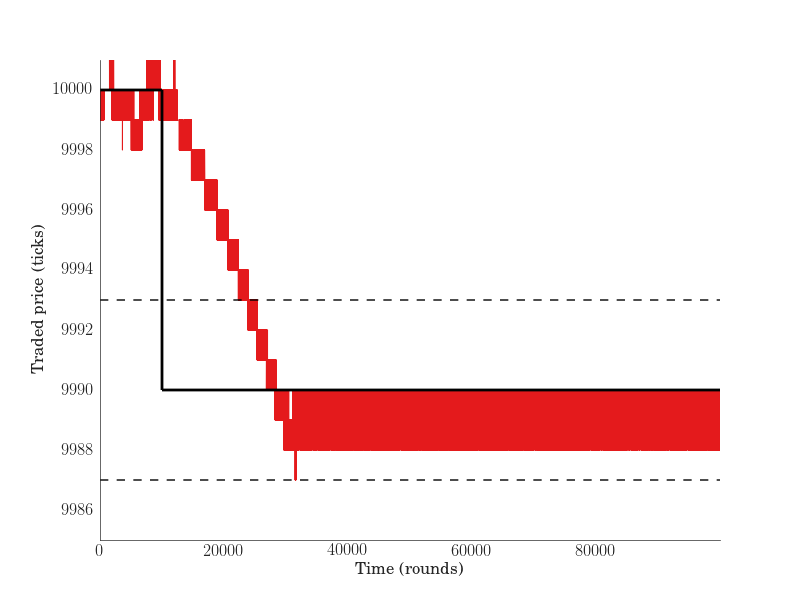
\includegraphics[width=0.5\textwidth]{figure_in_fitness_section/a_stable_within_margin.png}}
\subcaptionbox{Within margin, but with flickering}
[0.49\linewidth]{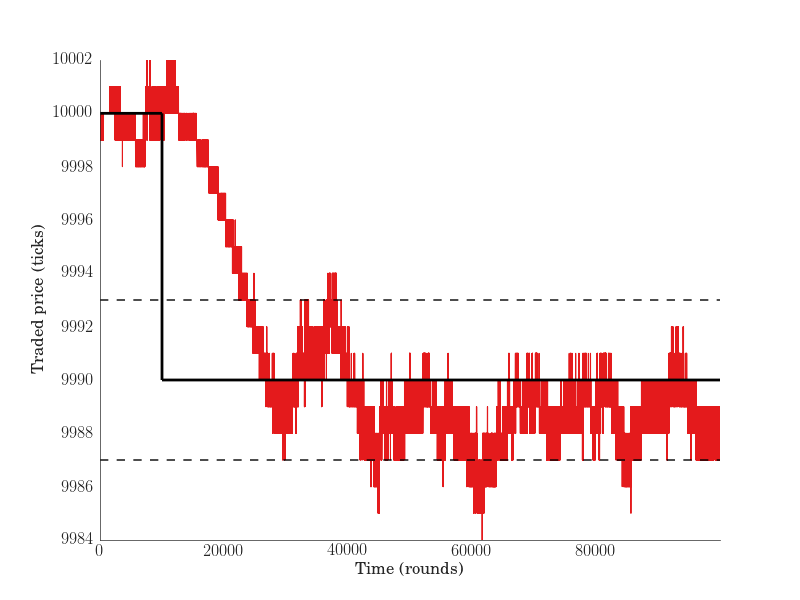
\includegraphics[width=0.5\textwidth]{figure_in_fitness_section/b_flicker_but_mostly_within_margin.png}}
\subcaptionbox{Flickering on the edge of margin}
[0.49\linewidth]{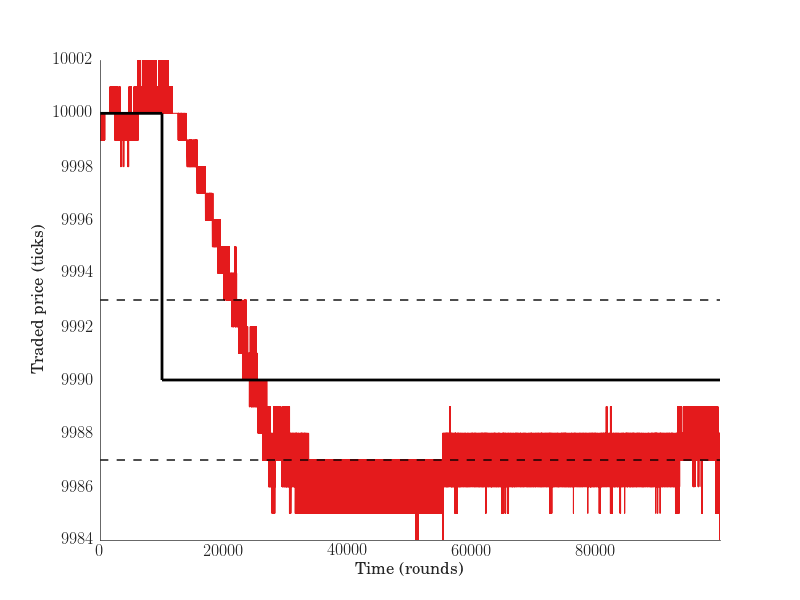
\includegraphics[width=0.5\textwidth]{figure_in_fitness_section/c_flickering_on_margin.png}}
\subcaptionbox{Never reach fundamental}
[0.49\linewidth]{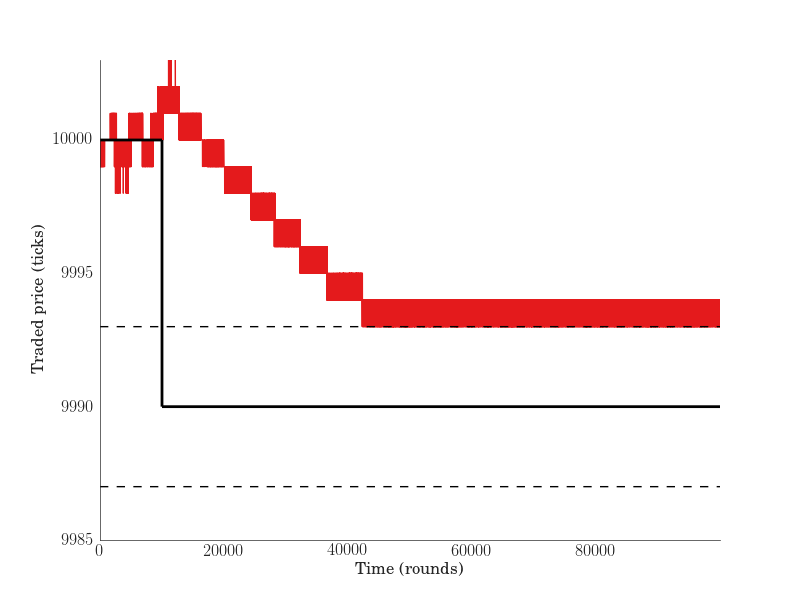
\includegraphics[width=0.5\textwidth]{figure_in_fitness_section/d_never_reach_fundamental.png}}
\subcaptionbox{Stabilize under fundamental}
[0.49\linewidth]{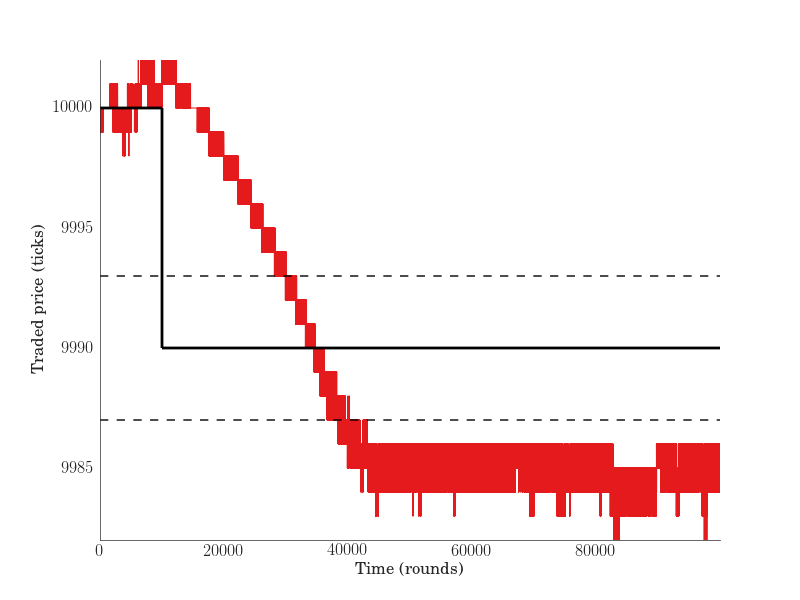
\includegraphics[width=0.5\textwidth]{figure_in_fitness_section/e_stable_under_fundamental.png}}
\subcaptionbox{Market crash}
[0.49\linewidth]{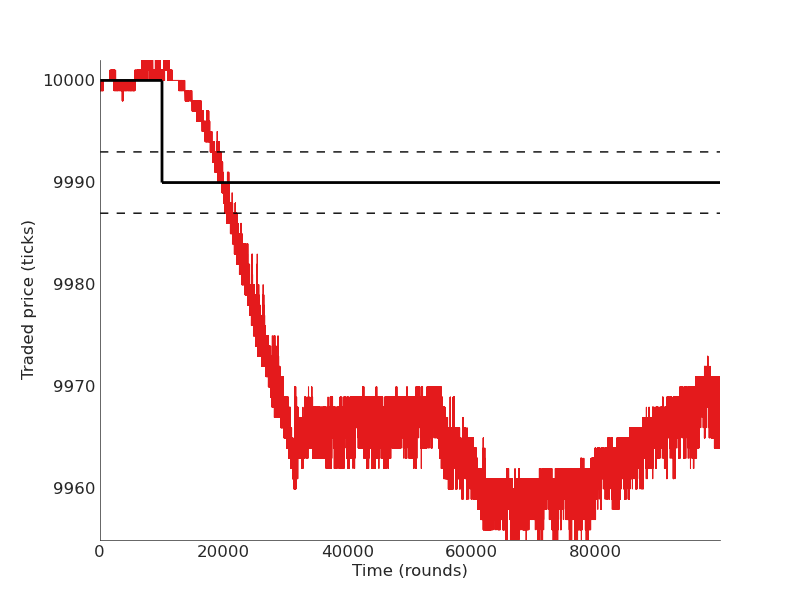
\includegraphics[width=0.5\textwidth]{figure_in_fitness_section/f_crash.png}}
\caption{Six examples of typical market dynamics}
\label{figure:typical_fitness_cases}
\end{figure}
%In particular the parameters controlling various time delays are of interest. 
%The search space of the parameters is very large, which makes an exhaustive search impossible.
%To this end, four fitness measures were defined.

%Several parameters influence the number of orders submitted by the high frequency traders.




\begin{comment}
\begin{figure}
\centering
\subcaptionbox{Market with fairly stable prices, but flickering over and under the stability margin. \label{figure:tradeprice_exaples_fitness_a}}
[0.49\linewidth]{\includegraphics[width=0.5\textwidth]{issue_113_tradeprice_plots/all/low_stdev_but_not_stable.png}}
\subcaptionbox{\label{figure:tradeprice_exaples_fitness_b}}
[0.49\linewidth]{\includegraphics[width=0.5\textwidth]{issue_113_tradeprice_plots/all/low_stdev_and_stable.png}}
\subcaptionbox{\label{figure:tradeprice_exaples_fitness_c}}
[0.49\linewidth]{\includegraphics[width=0.5\textwidth]{issue_113_tradeprice_plots/all/high_stdev_but_stable.png}}
\caption{title}
\label{figure:tradeprice_exaples_fitness}
\end{figure}
\end{comment}



\subsection{Configuring the genetic algorithm}\label{section:ga_parameters}
Although this is a basic version of genetic algorithm, using it correctly is not necessarily easy, as was encountered. First of all, the parameters for the genetic algorithm itself must be established. The larger and more complex the search space, the more resources the search will require, since the evaluating the fitness function (i.e., the running the simulation) will have to be performed a larger number of times. Table \ref{table:genetic_algorithm_parameters} presents an overview of the parameters used in the genetic algorithm. The tournament size was set to three, as this provided the best balance between diversification and speed of convergence \cite{blickle1995comparisonkeylist, goldberg1991comparative}, considering the high computational  of the model.

\begin{table}
	\centering
	\begin{tabular}{l|l}
		Parameter & Assignment\\\hline
		Number of individuals & 200\\
		Cross-over points & 2\\
		Tournament size & 3\\
		Mutation probability & 0.1\\
		Mutation distribution &  $\mathcal{N}(\mu = 0, \sigma = 0.1)$\\
	\end{tabular}
	\caption{Overview of parameters used in the genetic algorithm}
	\label{table:genetic_algorithm_parameters}
\end{table}



\subsection{Filtering parameters}\label{section:filtering_parameters}

The model parameters do influence the fitness values as they control model behavior, but they are not directly weighted into the fitness-values. This means that even after the parameters of the genetic algorithm was properly tuned in such a way that higher-fitness individuals were produced, these individuals often turned out to be of no interest. Such individuals were discarded according to the filtering criteria described in this section.

As mentioned earlier, it is not enough simply to define a fitness function which assigns high values to parameters causing realistic behavior. In addition, it is important to discard parameters which obviously do not correspond to a realistic setting. Imagine that the simulation scores high fitness values when executed without any market makers. Since it is known that real markets do in fact contain market makers, nothing can be inferred from such a result. Indeed this might be a consequence of poorly designed fitness measures, but since it is easier to use domain specific knowledge to filter out the unrealistic parameters


\begin{figure}
	%issue 15
	\subcaptionbox{Market with unrealistic parameters (no fast traders) with seemingly realistic dynamics\label{subfig:unrealistic_parameters}}
		[0.49\linewidth]{\includegraphics[width=0.5\textwidth]{manually_selected/no_agents.png}}
	\subcaptionbox{Parameters causing unrealistic dynamics\label{subfig:unrealistic_behavior}}
	[0.49\linewidth]{\includegraphics[width=0.5\textwidth]{manually_selected/crazy_market.png}}
	\caption{Two examples of why model parameters must be restricted}
\end{figure}
The first graph is an example of a simulation which is assigned fairly good fitness values, but which was executed with clearly unrealistic parameters: $\ssmmnAgents = \scnAgents = 0$. The simulation reaches the new fundamental price fairly quickly without any undershoot, and stays within the stability margin. The only point where it scores badly is the standard deviation which is slightly high due to the fluctuating trade price.

\section{Applying the genetic algorithm}
Applying the genetic algorithm to produce markets with desirable behavior turned out to be more difficult that one could have hoped for. First of all, the high computational costs was a hurdle. The high time complexity stems from several factors
\begin{itemize}
\item Running a simulation for a given set of parameters required up to several minutes of computation on a single CPU core.
\item Large number of model parameters increase the size of the search space. The more parameters Unfortunately there is no magic to the way the genetic algorithm works, and optimizing in a larger search means a larger time complexity.
\item Large range of parameters. Some of the parameters are integers while some are real numbers. While most of the parameters have a lower bound, none of the parameters have upper bounds.
\item Unstable fitness parameters. Since the same set of parameters can produce varying model behavior, the fitness-values may also vary. Therefore it is necessary to evaluate the simulation several times for each set of parameters. 
\item The model parameters also influence the time complexity. For instance, evaluating a simulation with many agents takes more time than evaluating a simulation with fewer agents. 
\end{itemize}
Genetic algorithms are naturally suited for parallel computation. Two servers with a total of 40 cores and enough memory to evaluate as many simulations were utilized. With this equipment, evaluating a single strategy (see section \ref{section:datasets_introduction})for generating data sets could take up to several weeks.


\subsection{Experiments: Dividing the search into parts}\label{section:datasets_introduction}
As mentioned earlier, the number of parameters and the range of each parameter influences the complexity of the search. Because of this, it is desirable to keep the number of parameters that are included in each individual as small as possible. However, fixing parameters means that some interesting properties about the model might not be discovered. Furthermore, varying all parameters at the same time makes the analysis and interpretation of the results more difficult. In an attempt to overcome this dilemma, several ``experiments'' were carried out \footnote{The reason for the quotes is that the term experiment might be stretching the common understanding of what an experiment is a little.}. Instead of trying to optimize all the model parameters at once, the search was split into several parts, each of which we call an experiment. Each of these experiments produce a data set, each of which were analyzed using the methods described in section \ref{section:data_analysis_techniques}. Some of the data sets produced interesting results, while others did not. Chapter \ref{chapter:results_and_discussion} focuses on the analysis and presents the findings. A brief overview of the experiments is presented in \ref{section:experiments_overview}, but since the motivation for creating each data set is best understood in the context of the analysis of each data set, the details are deferred until chapter \ref{results_and_discussion}. The next section will explain exactly what a data set is.

\subsection{Gene pool as data set}\label{section:gene_pool_as_data_set}
The previous sections contain the details of each of the steps undertaken in order to produce data sets. To summarize, the list below enumerates the steps.
\begin{enumerate}
\item Initialize a population in the genetic algorithm with healthy individuals.
\item Evaluate the fitness for every individual several times and obtain fitness-values by calculating averages.
\item Stack all individuals that ever lived into a $\datasetNpoints \times \individuallength$ parameter data matrix \datamatrixpar, where $\datasetNpoints$ is the number of individuals, and $\individuallength$ is the length of each individual. Likewise, stack the fitness values into a $\datasetNpoints \times \fitnesslength$ fitness-data matrix \datamatrixfit, where \fitnesslength is the number of fitness values calculated. 
\item Filter the data by removing rows in \datamatrixpar with parameters which can be deemed not to correspond to real markets, and by removing rows in \datamatrixfit with fitness values that are not realistic. Please refer to section \ref{section:filtering_parameters} for details. Naturally, when a row is removed in \datamatrixpar, it is also removed in \datamatrixfit, and vice versa. 
\item Likewise, data points which were generated by a simulation crashing before it could complete were removed.
\end{enumerate}
Tables \ref{table:example_dataset_parameters} and \ref{table:example_dataset_fitnesses} contain the first rows of \datamatrixpar and \datamatrixfit for one of the data sets.
\begin{table}
\centering
\small
\begin{tabular}{lrrrrrrrrrrrrrr}
\toprule
{} &  \sclatencymu &   \sclatencys &   \scnAgents &   \scthinkmu &   \scthinks &   \sctimehorizonmu &   \sctimehorizons &   \scwaitTimeBetweenTradingmu &   \scwaitTimeBetweenTradings &   \ssmmlatencymu &   \ssmmlatencys &   \ssmmnAgents &   \ssmmthinkmu &   \ssmmthinks \\
\midrule
0 &            84 &            11 &           14 &           98 &           9 &               1071 &               445 &                            38 &                           17 &                3 &               2 &             48 &              8 &             1 \\
1 &            23 &            21 &           74 &           49 &          24 &                529 &               554 &                            45 &                           13 &                9 &               0 &              8 &              5 &             3 \\
2 &            51 &            13 &           53 &           47 &          13 &               3586 &               536 &                            10 &                           11 &                9 &               4 &             14 &              4 &             2 \\
3 &            18 &            21 &          213 &           70 &          39 &                793 &              1179 &                            33 &                           15 &                7 &               2 &             43 &              6 &             3 \\
4 &            94 &            41 &          144 &           10 &          25 &               2668 &               893 &                            12 &                           15 &                6 &               1 &             49 &              7 &             4 \\
5 &            19 &             4 &          130 &           15 &          38 &               1085 &              1165 &                            39 &                            4 &                2 &               3 &             11 &              4 &             4 \\
6 &            65 &            15 &           91 &           81 &          46 &               3867 &              1991 &                            48 &                            1 &                7 &               2 &             21 &              4 &             4 \\
7 &            36 &            38 &          143 &           77 &          19 &               2805 &              1870 &                            10 &                            9 &                7 &               0 &              3 &              2 &             4 \\
8 &            43 &             8 &           10 &           19 &          19 &               3384 &              1706 &                            33 &                            4 &                8 &               4 &              5 &              5 &             0 \\
9 &            11 &            33 &          127 &           94 &          49 &               3597 &               723 &                            12 &                            2 &                7 &               1 &             33 &              5 &             4 \\
\bottomrule
\end{tabular}

\caption{An example data matrix containing the parameters of ten individuals who lived sometime during the execution of the genetic algorithm. In this case, each individual contained parameters for the number of HFT agents, as well as the latency and thinking time parameters. Hence, the data matrix has a column for each parameter.}
\label{table:example_dataset_parameters}
\end{table}
\begin{table}
\centering
\begin{tabular}{lrrrr}
\toprule
{} &  \overshoot &   \roundstable &    \stdev &   \timetoreachnewfundamental \\
\midrule
0 &           3 &          25359 &  0.382092 &                        29838 \\
1 &           7 &          99999 &  1.289659 &                        23373 \\
2 &           6 &          99999 &  1.253363 &                        18748 \\
3 &           7 &          99997 &  1.695150 &                        22819 \\
4 &           6 &          94343 &  1.329276 &                        22703 \\
5 &          16 &          99999 &  2.439084 &                        31860 \\
6 &           6 &          93378 &  1.287235 &                        25645 \\
7 &          10 &          99997 &  1.858166 &                        19417 \\
8 &           3 &          24039 &  0.935465 &                        27381 \\
9 &          19 &          99995 &  4.092439 &                        24845 \\
\bottomrule
\end{tabular}

\caption{This table contains the fitness values for each individual in table \ref{table:example_dataset_parameters}. Note that, in order to increase the reliability of the fitness measure of an individual, the recorded fitness-values are the average of the fitness-values obtained by evaluating each individual ten times}
\label{table:example_dataset_fitnesses}
\end{table}


\section{Data analysis techniques}\label{section:data_analysis_techniques}
Using inverse simulation creates a lot of data, which is aggregated into a data matrix as described in the previous section. This data has to be analyzed in order to obtain insight into how the various parameters, especially those concerning the latency of the fast traders, influence the market.


\subsection{Clustering algorithms}
Clustering methods were used to obtain representative nodes in both the fitness space and the parameter space. Clusters in \datamatrixfit{}{} partitioning the fitness space can be thought of as representing markets with different types of behavior. Likewise, clusters in \datamatrixpar{}{} represent markets in which various conditions are present. Ideally, there is a large overlap between the assignment of data points to the clusters in the fitness space and to clusters in the parameters space. Such overlaps will signify that markets in which certain conditions are present (such as a large number of fast market makers) will tend to have certain behaviors, and vice versa. \datamatrixpar{}{} can be thought of as a data matrix containing features, while \datamatrixfit{}{} can be thought of as a data matrix containing target variables. 

The benefit of this method over trying to train a regression model is that it is easier to interpret how parameters are mapped to fitness values by the model. Training, say, a neural network might indeed enable us to make predictions of the market behavior given a set of parameters. However, the goal of this thesis is not to make predictions of market behavior within the model, but rather to understand how certain parameters influence the market behavior. Hence there is no need to employ modeling techniques that are more complex that they have to be. 

Three different clustering techniques were used in this work. The motivation for employing each of these techniques is described below. All three clustering algorithms are implemented as part of the \texttt{scikit-learn} toolkit\cite{pedregosa2011scikit}.

\begin{description}
\item[K-means clustering (KM)] K-means clustering is probably the most widely used clustering algorithm, and performs well complexity-wise even on reasonably large data sets. The algorithm requires the specification of the number of clusters, which can be a disadvantage. K-means clustering minimizes an objective function (or distortion measure \cite{bishop2006pattern}) calculated as the sum of squared distances between the points and their assigned clusters. It is important to note that the assignment of points to clusters is not guaranteed to yield the global minimum of the objective function \cite{izenman2008modern}. The clustering was therefore run several times, and the assignment with the lowest distortion is used. In order to speed up the calculation, the Mini-Batch version of the clustering algorithm was used \cite{sculley2010web}.
\item[Affinity propagation] This algorithm has the benefit that it does not require the specification of a number of clusters \cite{frey2007clustering}. Since the algorithm has problems dealing with large data sets, K-means clustering was used to reduce the number of data points by using 1000 clusters as representatives of the data.
\item[Gaussian mixture model (GMM)] The Gaussian mixture model is another incredibly popular clustering algorithm since it is both fast and can calculate complex decision boundaries\footnote{Another delicious property of the model is that it is generative, although this property was not used in this work}. When the model is allowed to a full covariance matrix, the number of parameters scales quadratically with the dimensionality of the data set, and this might lead to gross over-fitting and the well-known problem of some of the clusters having variances approaching zero. However, as \datamatrixfit{} has only four dimensions and several hundreds of thousands of data points, the GMM can be safely allow to have a full covariance matrix. The GMM was fitted used the EM-algorithm \cite{bilmes1998gentle, bishop2006pattern}.
\end{description}

The best algorithm for dealing with the problem at hand turned out to be the GMM algorithm, for reasons which are discussed in section \ref{section:clustering}. All three clustering algorithms are sensitive to outliers, and the next section discussed the two methods used for dealing with such data points.




\subsection{Preprocessing}
Each experiment generated two data matrices, \datamatrixfit{}{} and \datamatrixpar{}. The dimensionality of \datamatrixfit{} is always equal to four, since only four fitness measures were defined, whereas the dimensionality of \datamatrixpar{}{} depends on how many parameters were included in the individuals of the genetic algorithm. Hence, in order to visualize how the data is distributed, the dimensionality must be reduced. Furthermore, since the data set contained abnormal data points, these had to be identified and removed.


\subsubsection{Normalization and dimensionality reduction}
The three clustering algorithms utilized all have problems with data sparsity. However, since \datamatrixfit{} only has four features, the data set poses no challenge to the clustering algorithms used. Instead, dimensionality reduction was used for the benefit of visualization. Principal component analysis was chosen. As the four fitness measures had very different ranges, the data in \datamatrixfit{} was normalized by subtracting the mean and dividing by the standard deviation, as in \cite{salkind2010encyclopedia}.

\subsubsection{Identifying outliers}\label{section:outliers}
The term outliers is often used as a label for data which is considered ``invalid'' in the sense that is not a product of the true data generation process, but has been corrupted by various sources of noise. In this report, data that was caused by failing simulations corresponds to the usual understanding of outliers. However, as was already explained in section \ref{section:failed_simulations}, data from such simulations are never included in \datamatrixpar{} and \datamatrixfit{} to begin with. Instead, outliers in this report refer to entries in \datamatrixpar{} and \datamatrixfit{}  deviate significantly from the majority of the data points by having extreme values.

Such data points caused problems when applying data analysis techniques which rely on a fairly normal distribution of the data points, such as Principal Component Analysis (PCA). PCA looks for a rotation of the data space, such that the axes of the new basis are aligned with the directions of the largest variance in the original space. Since a few points with extreme values come to account for a large portion of the data set variance, the new basis computed by PCA will be aligned along these few data points. When PCA is used to extract lower dimensional features from the data set, outliers will degrade the quality of these features. In the case that PCA is used for data visualization, the scatter plots of the first few principal components will not be very informative, as they merely show the projection of the data onto the axes aligned with the outliers.

In all experiments, outliers were present in both the parameters space and in the fitness space. Outliers in the parameter space occur because of abnormally large mutations, and any dimension of the parameter space is susceptible to such an event. In the fitness space, only a few of the features suffered from the occurrence of outliers. The feature \roundstable cannot contain outliers, because the shock to the fundamental occurs at round $\round = 10^4$, and because the simulation is terminated at round $\round = 10^5$, hence $\roundstable \in [10^4,10^4+1,\hdots 10^5]$. The same is true for \timetoreachnewfundamental. \stdev and \overshoot, on the other hand, are susceptible to outliers, because the two features have no upper bound. Note that markets with abnormally large overshoot are interesting in themselves, as something caused these markets to crash. However, since the clustering algorithms are sensitive to the presence of data points that deviate significantly from the majority of data, such data points are removed. 

\begin{enumerate}
\item Apply a monotonically increasing transformation $f(x)$ to some or all of the features for every data point in the data set. A common choice of $f$ is $f(x) = \log x$, as it efficiently reduces the impact of data points with extremely high values. Figure \ref{figure:scatter_log_transform} illustrates the effect of applying the log-transform. The log-scaling does a fairly good job of reducing the importance of the outliers in the \stdev feature, while the change is less dramatic in \timetoreachnewfundamental. While the left scatter plot does not really reveal any structure of the data, the transformation makes it possible to spot to rough clusters when inspecting the right plot.
\item Manually select one or more criteria for when a data point is to be considered an outlier. 
%\item Use a one-class support vector machine to calculate a probability for each data point that said point is an inlier or an outlier. 
\end{enumerate}




%In the parameters data set, outliers can occur due to abnormally large mutations. 
%Some parameters cause the simulation to act in strange ways, and even crash in some cases. For instance, the the order book becomes empty, the simulation throws an exception and terminates. Similarly, if the best \bid/\ask prices drops to zero, the simulation exits. As such 